\documentclass[12pt]{article} % use larger type; default would be 10pt

\usepackage[utf8]{inputenc} % set input encoding (not needed with XeLaTeX)

%%% PAGE DIMENSIONS
\usepackage{geometry} % to change the page dimensions
\geometry{a4paper} % or letterpaper (US) or a5paper or....
%\geometry{margins=1in} % for example, change the margins to 2 inches all round
% \geometry{landscape} % set up the page for landscape
% read geometry.pdf for detailed page layout information

\usepackage{graphicx} % support the \includegraphics command and options

%\usepackage[parfill]{parskip} % Activate to begin paragraphs with an empty line rather than an indent

%%% PACKAGES
\usepackage{booktabs} % for much better looking tables
\usepackage{array} % for better arrays (eg matrices) in maths
\usepackage{paralist} % very flexible & customisable lists (eg. enumerate/itemize, etc.)
\usepackage{verbatim} % adds environment for commenting out blocks of text & for better verbatim
\usepackage{subfig} % make it possible to include more than one captioned figure/table in a single float
\usepackage{amsmath}
\usepackage[]{mcode}
% These packages are all incorporated in the memoir class to one degree or another...


%%% HEADERS & FOOTERS
\usepackage{fancyhdr} % This should be set AFTER setting up the page geometry
\pagestyle{fancy} % options: empty , plain , fancy
\renewcommand{\headrulewidth}{0pt} % customise the layout...
\lhead{}\chead{}\rhead{}
\lfoot{}\cfoot{\thepage}\rfoot{}

%%% END Article customizations

\begin{document}

\noindent
Joe Sinotte

\vspace{3mm}
\begin{center}
Final Project
\end{center}

\vspace{3mm}
\noindent
\textbf{Statement of the Problem:}

\vspace{3mm}
Given a data set, in this case a binary and Markovian sequence, and a noisy observation of the data, is it possible to reconstruct the original data from the noisy observation?

\vspace{5mm}
\noindent
\textbf{Data:}

\vspace{3mm}
As stated above, the data set used will be a binary Markovian sequence. Here, I will construct a variable $x = (x_{1}, \cdots, x_{n})$ according to the following:  

\vspace{2mm}
\[
x_{1} = 
\begin{cases}
0 & \text{with probability } 0.5 \\
1 & \text{with probability } 0.5
\end{cases}
\]

\vspace{5mm}

\[
x_{i} =
\begin{cases}
x_{i-1} & \text{with probability} \hspace{1mm} p \\
1-x_{i-1} & \text{with probability} \hspace{1mm} 1-p
\end{cases}
\]

\vspace{3mm}
Having generated the sequence of variables that will be used, the next step is to define a noisy observation of x, where the variable is observed with some error possible. This noisy variable will be defined as:

\begin{center}
$y_{i} = x_{i} +e_{i}$
\end{center}

\noindent
where, 

\begin{center}
$e_{i} \sim N(0, \sigma^{2})$
\end{center}

\begin{center}
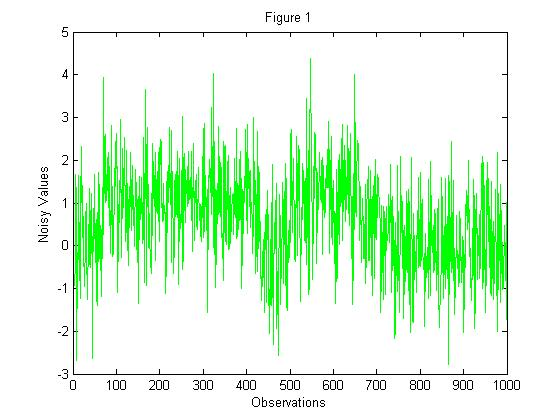
\includegraphics[scale=.35]{figure1}
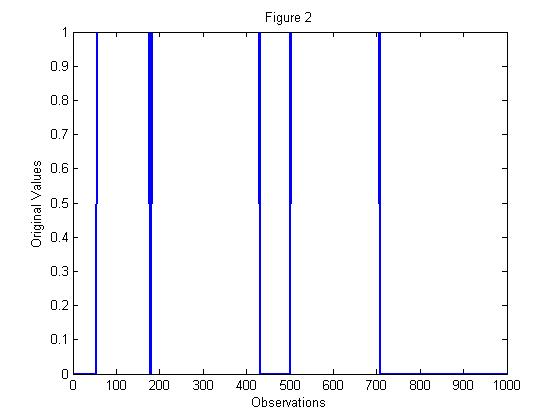
\includegraphics[scale=.35]{figure2}
\end{center}

\vspace{3mm}
Figure 1 shows the values of the noisy observations and Figure 2 shows the original values of x. Both sets of variables were constructed according to the definitions above. Having constructed both sets of data, the goal of this exercise is now to determine whether or not the original data, x, can be reconstructed from the noisy data, y. In the sections to follow, I will describe the methodology used to approach this problem.

\vspace{3mm}
\noindent
\textbf{Dynamic Programming:}

\vspace{3mm}
This project made use of an important computational tool called dynamic programming, which can be used to find optimal trajectories in situations where the decisions are made in stages, and decisions made in past stages have future consequences.

\vspace{3mm}
The particular method used to reconstruct the data is called the Maximum A Posteriori Method. This method involves taking a noisy observation and using a maximum likelihood technique to guess the most likely value for the reconstructed variable, given the observation. This process can be expressed mathematically as:

\begin{equation*}
\{z_{i}\} = argmax \hspace{1mm} Pr(\{ x_{i} \} \vert \{y_{i} \}) = argmax \hspace{1mm} log(Pr(\{x_{i}\} \vert \{y_{i}\}))
\end{equation*}

\vspace{3mm}
\noindent
Which can be stated alternatively as:

\begin{equation*}
= argmax \hspace{1mm} \sum_{i = 1}^{N} \Big( - \frac{(y_{i} - x_{i})^{2}}{2 \sigma^{2}} \Big) + \sum_{i=2}^{N} log(1_{x_{i} = x_{i-1}} p + 1_{x_{i} \neq x_{i-1}} (1-p))
\end{equation*}

\vspace{3mm}
Hence, the values of z will denote the reconstructed variables which are compiled by maximizing the probability of the variable, x, conditioned on the observed noisy variable, y.


\vspace{3mm}
\noindent
\textbf{Results:}

\vspace{3mm}
In the first portion of this exercise, the values for p and $\sigma$ were set to $0.99$ and $1$, respectively. Then, using the Maximum A Posterior method described above, a dynamic program was implemented in Matlab to compute the reconstructed variable, z, from the noisy variable, y. This program was run 5 times and the rate of success for each iteration was computed as the proportion of reconstructed variables that matched the original variables, x. The average rate of success over these 5 iterations is given as:

\begin{equation*}
average1 = 0.9798
\end{equation*}

\begin{center}
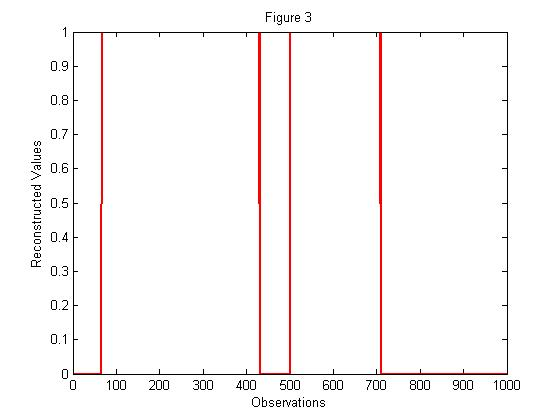
\includegraphics[scale = .35]{figure3}
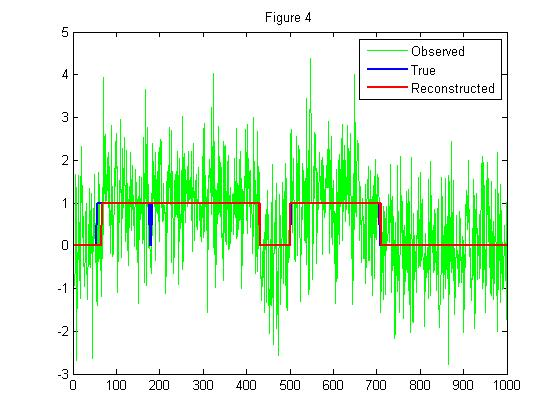
\includegraphics[scale = .35]{figure4}
\end{center}

Figure 3 shows the reconstructed values, and Figure 4 shows the original values, x, the noisy values, y, and the reconstructed values, z, for the 5th iteration. Figure 4 as well as the average success rate reported above serve to demonstrate that this exercise was largely successful, but for few errors.

\vspace{3mm}
For the next portion of this project, I allow the values of p to vary while maintaining that $\sigma = 1$. Specifically, I will define p to be:

\vspace{1mm}
\begin{equation*}
p = [0.9 \hspace{3mm} 0.8 \hspace{3mm} 0.7 \hspace{3mm} 0.6]
\end{equation*}

\vspace{3mm}
For each value of p, five repetitions were run and the average success rate was computed as before. Figure 5 shows these average success rates across the four possible values of p. As the figure shows, a smaller level of p corresponds to a lower probability of success. This is because as p gets smaller, it becomes more likely that x changes between observations, inducing more variation in the data and making it more difficult to successfully reconstruct values for z.

\begin{center}
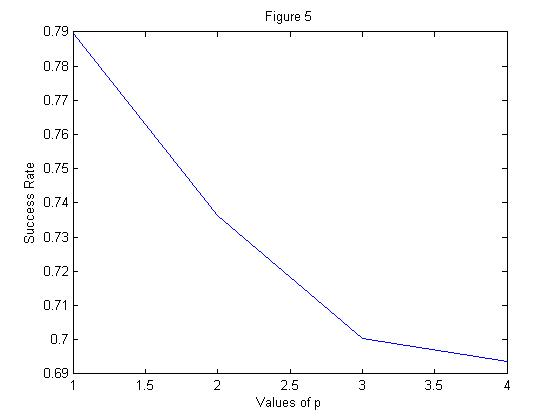
\includegraphics[scale = 0.5]{figure5}
\end{center}

For the final portion of this project, I set $p = 0.99$ and allow the values of $\sigma$ to vary. Specifically, I define $\sigma$ as:

\begin{equation*}
\sigma = [0.5 \hspace{3mm} 1 \hspace{3mm} 2 \hspace{3mm} 5]
\end{equation*}

\vspace{3mm}
For each value of $\sigma$, five repetitions were run and the average success rate was computed as before. Figure 6 shows these average success rates across the four possible values of $\sigma$. As the figure shows, a higher value for $\sigma$ corresponds to a lower probability of success. This is because as $\sigma$ gets smaller, the values of the noisy observations have greater variance making it more difficult to successfully reconstruct values for z.

\begin{center}
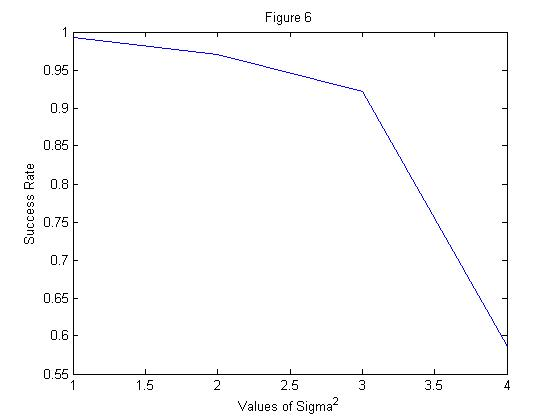
\includegraphics[scale = 0.5]{figure6}
\end{center}

\vspace{3mm}
\noindent
\textbf{Conclusion:}

\vspace{3mm}
Overall, this exercise was successful. Using, the Maximum A Posterior Method, I have shown that reconstructed values can be found from noisy observations. In the process, I have also found that as the value of p decreases, it becomes more difficult to successfully reconstruct the data. Additionally, as the value of $\sigma$ increases, it becomes more difficult to reconstruct the data.

\pagebreak
\noindent
\textbf{Matlab Program:}

\begin{lstlisting}
%%%%%%%%%%%%%%%%%%%%%%%%%%%%%%%%%%%%%%%%%%%%%%%%%%%%%%%%%%%%%%%%%%%%%%%%%%%
%%%%%%%%%%%%%%%%%%%%%%%%%%%% Final Project %%%%%%%%%%%%%%%%%%%%%%%%%%%%%%%%
%%%%%%%%%%%%%%%%%%%%%%%%%%%%%%%%%%%%%%%%%%%%%%%%%%%%%%%%%%%%%%%%%%%%%%%%%%%

clear
clc

N = 1000;
sigma = 1;
p = .99;

for i = 1:5
    
    %%%% Generate Initial Value of x
    x(1) = (rand < .5);
    
    %%%% Generate Remaining Values of x
    for j = 2:N
        if rand < p
            x(j) = x(j-1);
        else
            x(j) = 1-x(j-1);
        end
    end
    
    %%%% Generate Noisy Observations
    for k =1:N
        y(k) = x(k)+normrnd(0,sigma);
    end
    
    %%%%%%%%%%%%%%%%%%%%%%%%%%%%%%%%%%%%%%%%%%%%%%%%%%%%%%%%%%%%%%%%%%%%%
    %%%%%%%%%%%%%%%%%%%%%%%%%%%%% Pseudo Code %%%%%%%%%%%%%%%%%%%%%%%%%%%
    %%%%%%%%%%%%%%%%%%%%%%%%%%%%%%%%%%%%%%%%%%%%%%%%%%%%%%%%%%%%%%%%%%%%%
    
    %%% Step 1
    
    s(1,1) = -(y(1)^2)/(2*sigma^2);
    s(1,2) =-((y(1)-1)^2)/(2*sigma^2);
    
    %%% Step 2
    
    for k = 2:N
        for j = 1:2
            h(1) = s(k-1,1) - .5/sigma^2*(y(k)-(j-1))^2 + log((j==1)*p
														+ (j==2)*(1-p));
            h(2) = s(k-1,2) - .5/sigma^2*(y(k)-(j-1))^2 + log((j==2)*p
														 + (j==1)*(1-p));
            
            if h(1) > h(2)
                b(k,j) = 0;
                s(k,j) = h(1);
            else
                b(k,j) = 1;
                s(k,j) = h(2);
            end
        end
    end
    
    %%% Step 3
    
    z(N) = (s(N,1) < s(N,2));
    for k=N-1:-1:1
        z(k) = b(k+1,z(k+1)+1);
    end
    
    for k = 1:1000
        if z(k) == x(k)
            S(k) = 1;
        else
            S(k) = 0;
        end
        s = sum(S);
    end
    
    success(i) = s/N;
    average1 = mean(success)
end





figure(1); clf; 
plot(1:N, y, 'g'); hold on;
plot(1:N, x, 'b', 'linewidth', 2);
plot(1:N, z, 'r', 'linewidth', 2);
legend('Observed', 'True', 'Reconstructed');






N = 1000;
sigma = 1;
p = [.9 .8 .7 .6];

for m = 1:4
    
    for i = 1:5
        
        %%%% Generate Initial Value of x
        x(1) = (rand < .5);
        
        %%%% Generate Remaining Values of x
        for j = 2:N
            if rand < p(m)
                x(j) = x(j-1);
            else
                x(j) = 1-x(j-1);
            end
        end
        
        %%%% Generate Noisy Observations
        for k =1:N
            y(k) = x(k)+normrnd(0,sigma);
        end
        
        %%%%%%%%%%%%%%%%%%%%%%%%%%%%%%%%%%%%%%%%%%%%%%%%%%%%%%%%%%%%%%%%%
        %%%%%%%%%%%%%%%%%%%%%%%%%%%%% Pseudo Code %%%%%%%%%%%%%%%%%%%%%%%
        %%%%%%%%%%%%%%%%%%%%%%%%%%%%%%%%%%%%%%%%%%%%%%%%%%%%%%%%%%%%%%%%%
        
        %%% Step 1
        
        s(1,1) = -(y(1)^2)/(2*sigma^2);
        s(1,2) =-((y(1)-1)^2)/(2*sigma^2);
        
        %%% Step 2
        
        for k = 2:N
            for j = 1:2
                h(1) = s(k-1,1) - .5/sigma^2*(y(k)-(j-1))^2 
								+ log((j==1)*p(m) + (j==2)*(1-p(m)));
                h(2) = s(k-1,2) - .5/sigma^2*(y(k)-(j-1))^2
								+ log((j==2)*p(m) + (j==1)*(1-p(m)));
                
                if h(1) > h(2)
                    b(k,j) = 0;
                    s(k,j) = h(1);
                else
                    b(k,j) = 1;
                    s(k,j) = h(2);
                end
            end
        end
        
        %%% Step 3
        
        z(N) = (s(N,1) < s(N,2));
        for k=N-1:-1:1
            z(k) = b(k+1,z(k+1)+1);
        end
        
        for k = 1:1000
            if z(k) == x(k)
                S(k) = 1;
            else
                S(k) = 0;
            end
            s = sum(S);
        end
        
        success(i) = s/N;
    end
    average2(m) = mean(success)
end

figure(2)
plot(average2)



N = 1000;
sigma = [.5 1 2 5];
p = .99;

for m = 1:4
    
    for i = 1:5
        
        %%%% Generate Initial Value of x
        x(1) = (rand < .5);
        
        %%%% Generate Remaining Values of x
        for j = 2:N
            if rand < p
                x(j) = x(j-1);
            else
                x(j) = 1-x(j-1);
            end
        end
        
        %%%% Generate Noisy Observations
        for k =1:N
            y(k) = x(k)+normrnd(0,sigma(m));
        end
        
        %%%%%%%%%%%%%%%%%%%%%%%%%%%%%%%%%%%%%%%%%%%%%%%%%%%%%%%%%%%%%%%
        %%%%%%%%%%%%%%%%%%%%%%%%%%%%% Pseudo Code %%%%%%%%%%%%%%%%%%%%%
        %%%%%%%%%%%%%%%%%%%%%%%%%%%%%%%%%%%%%%%%%%%%%%%%%%%%%%%%%%%%%%%
        
        %%% Step 1
        
        s(1,1) = -(y(1)^2)/(2*sigma(m)^2);
        s(1,2) =-((y(1)-1)^2)/(2*sigma(m)^2);
        
        %%% Step 2
        
        for k = 2:N
            for j = 1:2
                h(1) = s(k-1,1) - .5/sigma(m)^2*(y(k)-(j-1))^2
										 + log((j==1)*p + (j==2)*(1-p));
                h(2) = s(k-1,2) - .5/sigma(m)^2*(y(k)-(j-1))^2
										 + log((j==2)*p + (j==1)*(1-p));
                
                if h(1) > h(2)
                    b(k,j) = 0;
                    s(k,j) = h(1);
                else
                    b(k,j) = 1;
                    s(k,j) = h(2);
                end
            end
        end
        
        %%% Step 3
        
        z(N) = (s(N,1) < s(N,2));
        for k=N-1:-1:1
            z(k) = b(k+1,z(k+1)+1);
        end
        
        for k = 1:1000
            if z(k) == x(k)
                S(k) = 1;
            else
                S(k) = 0;
            end
            s = sum(S);
        end
        
        success(i) = s/N;
    end
    average3(m) = mean(success);
end

figure(3)
plot(average3)
\end{lstlisting}



\end{document}